\documentclass[aspectratio=169,usenames,dvipsnames]{beamer}
\usepackage{preamble}
\title{Coding for Humanities, week 1}
\begin{document}

\begin{frame}
 \titlepage
\end{frame}

\begin{frame}{Plan for today}
 \tableofcontents
\end{frame}




\section{Why programming}
\frame{\tableofcontents[currentsection]}
\begin{frame}{Programming: informal understanding}
    \begin{reference}
        Pine (2009). Learn to program. \url{https://pine.fm/LearnToProgram}
    \end{reference}
    \begin{definition}
        ``\structure{Programming} is telling your computer
        how to do something'' (Pine 2009, xii)
    \end{definition}
\end{frame}

\begin{frame}
    Why use computers in research?
	\pause

    \begin{itemize}
        \item Automation
        \item Amplification
        \item Reproducibility
    \end{itemize}

    \pause
    Computers need to be told what to do:

    \begin{itemize}
    \item Either user tools designed for a particular job
        \begin{itemize}
            \item but: limited to existing functionality
            \item cannot easily repeat a sequence of actions
        \end{itemize}

    \item \dots or create your own programs
        \begin{itemize}
            \item Higher investment to get started
            \item \dots but opens up lots of opportunities
        \end{itemize}
    \end{itemize}
\end{frame}

\begin{frame}{Research workflow}
    \begin{enumerate}
        \item Formulate research question
        \item Collect data
        \item Pre-process data
        \item Analyze data
        \item Draw conclusions
    \end{enumerate}

    \pause
    \dots programming is useful for steps 2--4
\end{frame}

\begin{frame}{Requirements for being a good programmer}
    \begin{itemize}
        \item Anyone can learn how to program
        \item Programming is a challenging activity:
            \begin{itemize}
                \item Meticulous analytic thinking
                \item Mental model of your program
                \item Paying attention to detail
            \end{itemize}
        \item Not everyone has the talent to become
            a \structure{good} programmer
    \end{itemize}
\end{frame}



\subsection{Example DH projects}
\begin{frame}{Example DH projects}
\begin{reference}
\url{https://twitter.com/yaelnetzer/status/1158712777776730113}
\end{reference}
    Student projects from a DH course by Yael Netzer (Israel):
    \begin{itemize}
        \item How many black actors/directors/producers are in movies?
        \item Which terror attacks are reported in the NY times?
        \item Sentiment analysis of GoodReads reviews vs NY times reviews
        \item Game of Thrones character analysis
        \item Eurovision song festival voting by country
    \end{itemize}
\end{frame}

\begin{frame}{Gender in Game of Thrones}\centering
    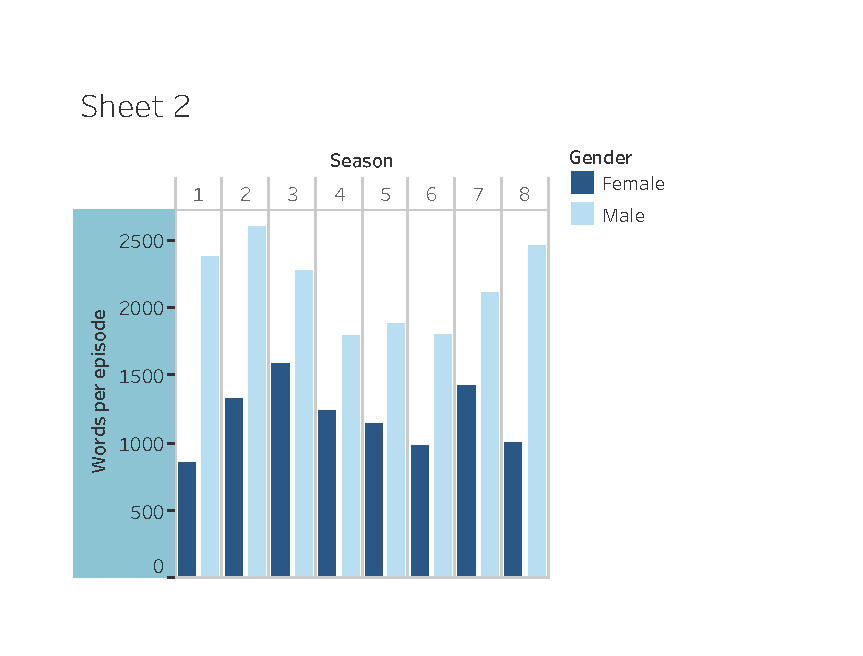
\includegraphics[width=0.6\textwidth]{fig/got}

    Words spoken for each gender across seasons
\end{frame}


\begin{frame}{``Don't let your dreams be dreams'' (Shia LeBeouf)}\centering
	\begin{reference}
		\url{https://www.youtube.com/watch?v=ZXsQAXx_ao0}
	\end{reference}
   
\includegraphics[width=0.6\textwidth]{fig/nothingisimpossible}
\end{frame}




\begin{frame}{Why Python}
    %\begin{definition}
    %   Python is a  ...
    %\end{definition}
    \begin{itemize}
        \item Easy and intuitive language:
            \begin{itemize}
                \item Code that is understandable as plain English
                \item Ease of development more important than fast programs
            \end{itemize}
        \item Suitable for many tasks:\\
            Many useful libraries (especially data science)
    \end{itemize}

    (Named after the TV show Monty Python)
\end{frame}

\begin{frame}
	% \begin{reference}
	% 	\href{https://www.economist.com/graphic-detail/2018/07/26/python-is-becoming-the-worlds-most-popular-coding-language}{
	% 		The Economist (2018): ``Python is becoming the world's most popular coding language''}
	% \end{reference}

    \centering
    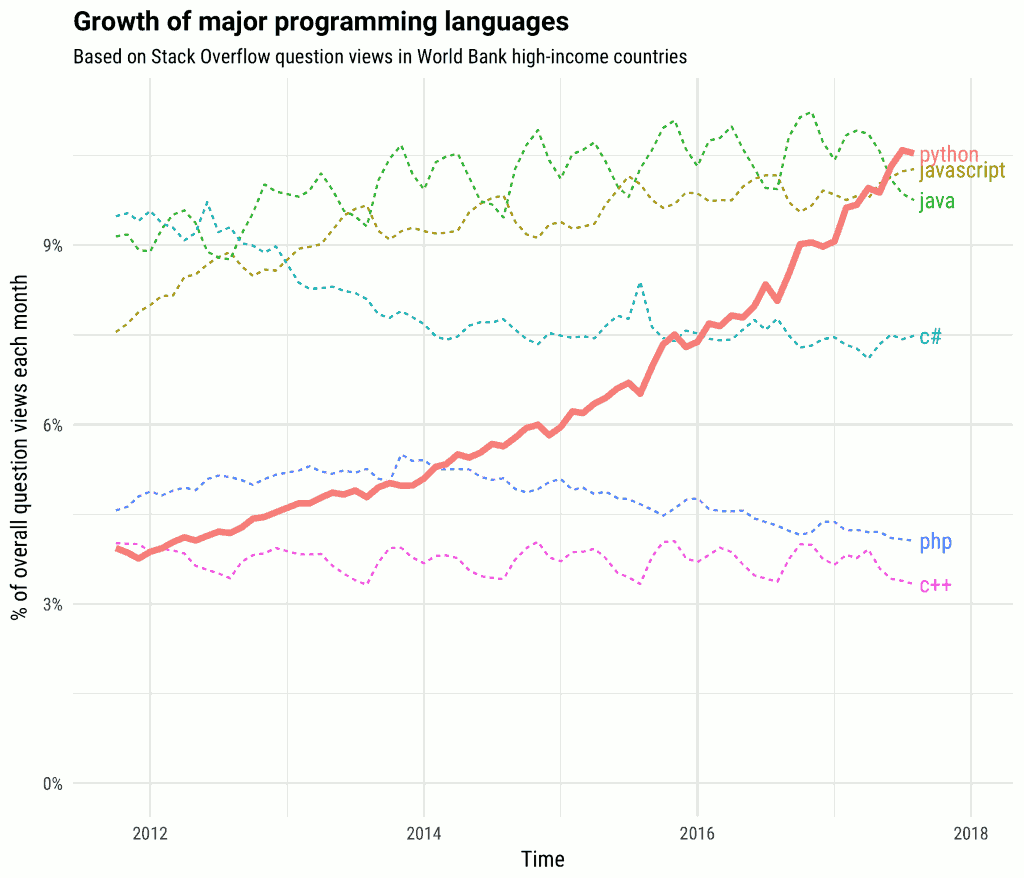
\includegraphics[height=0.9\textheight]{fig/pythongrowth.png}

    Source: \url{https://stackoverflow.blog/2017/09/06/incredible-growth-python/}
\end{frame}

\begin{frame}[fragile]
A simple Python program:
\begin{lstlisting}[language=python]
print('Hello, World!")
\end{lstlisting}

\pause
\vspace{1em}
The same program in the Java programming language:

\begin{lstlisting}[language=java]
public class HelloWorld {
    public static void main(String[] args) {
        System.out.println("Hello, World!");
    }
}
\end{lstlisting}
\end{frame}


\begin{frame}
	\begin{columns}
		\column{0.5\linewidth}
			Traditional method:
			\begin{enumerate}
				\item edit file
				\item run
				\item repeat
			\end{enumerate}
		\column{0.5\linewidth}
			Notebooks
			\begin{itemize}
				\item Notebook: combines text, code, and results
				\item Graphical interface in browser
			\end{itemize}
			[demo of Jupyter notebook]
	\end{columns}
\end{frame}



\section{Programming fundamentals}
\subsection{Numbers, text, and variables}
\frame{\tableofcontents[currentsection]}

\begin{frame}[fragile]{Using Python as a calculator}
Operators:
    \begin{description}
        \item[Addition] 1 + 2
        \item[Subtraction] 2 - 1
        \item[Multiplication] 2 * 3
        \item[Division] 6 / 2
        \item[Exponentation] 3 ** 2
        \item[Parentheses] (1 + 2) * 3
    \end{description}
\end{frame}

\begin{frame}[fragile]{Using Python as a calculator}
One or more operators can be used to form an \structure{expression}
\begin{lstlisting}[language=python]
>>> 1 + 2 * 3
7
>>> (1 + 2) * 3
9
\end{lstlisting}

\pause
Note: just as in mathematics, multiplication/division takes precedence over
    addition/subtraction. Parentheses can be used to specify a different order.
\end{frame}

\begin{frame}[fragile]{Numeric data types}
    \begin{description}
        \item[Integer] whole numbers: 1, 2, 3, \dots -1, -2, -3
        \item[Floating point] numbers: 2.5, 1.3333, \dots
    \end{description}

\pause
\begin{lstlisting}[language=python]
>>> 5 / 2
2.5
>>> type(5 / 2)
<class 'float'>
>>> type(6 / 2)
<class 'int'>
\end{lstlisting}
\end{frame}

\begin{frame}[fragile]{Variables}
    \begin{definition}
        A \structure{variable} stores the result of an expression
        so that it can be re-used.
    \end{definition}

A variable is created/updated using `=':

\begin{definition}
\structure{Assignment}: \texttt{name = expression}

The name consists of one or more letters or underscores (case-sensitive).
\end{definition}

\begin{lstlisting}[language=python]
>>> a = 5 / 2
>>> a
2.5
\end{lstlisting}
\end{frame}

\begin{frame}[fragile]{Using variables}
Now, can use variable in expressions in place of a number:

\begin{lstlisting}[language=python]
>>> a + 0.5
3.0
\end{lstlisting}

\pause
A program is executed line-by-line, and variables can be overwritten:
\begin{lstlisting}[language=python]
>>> a = 2
>>> a
2
>>> a = 3
>>> a
3
\end{lstlisting}
\end{frame}


\begin{frame}[fragile]{Updating variables}
A common operation is to increase the value of a variable:
\begin{lstlisting}[language=python]
>>> a = 2
>>> a = a + 1
3
\end{lstlisting}

\pause
There is a shorthand for this operation:
\begin{lstlisting}[language=python]
>>> a = 2
>>> a += 1
3
\end{lstlisting}

Also -=, *=, etc.
\end{frame}


\begin{frame}[fragile]{A practical example}
    Suppose I read War \& Peace in a year,
    what is my reading speed (words per minute)?
    \begin{itemize}
        \item Number of words in War \& Peace: 564,277
        \item Time spent reading per day: 1 hour
    \end{itemize}
    How to calculate average words per minute?
    \pause

\begin{lstlisting}[language=python]
>>> words_per_day = 564277 / 365
>>> words_per_min = words_per_day / 60
>>> words_per_min
25.766073059360732
\end{lstlisting}
\end{frame}

\begin{frame}[fragile]{Text}
Values can also be text instead of numbers:
\begin{lstlisting}[language=python]
>>> name = 'John'
>>> movie = '2001: A Space Odyssey'
\end{lstlisting}

\pause
    \begin{definition}
        A \structure{string}, short for string of characters,
        is a type of value that contains text.
    \end{definition}
\end{frame}

\begin{frame}[fragile]{Operations on strings}
\begin{lstlisting}[language=python]
>>> first = 'John'
>>> last = 'Doe'
\end{lstlisting}
\begin{description}
    \item[first + last] \texttt{'JohnDoe'}
    \item[first - last] TypeError
    \item[first * last] TypeError
    \item[first / last] TypeError
\end{description}

\begin{itemize}
\item + can be used to concatenate two strings
\item The other operations require numbers, not text
\end{itemize}
\end{frame}

\begin{frame}[fragile]{Mixing strings and numbers}
\begin{lstlisting}[language=python]
>>> first = 'John'
>>> num = 3
\end{lstlisting}
\begin{description}
    \item[first + num] TypeError
    \item[first - num] TypeError
    \item[first * num] 'JohnJohnJohn'
    \item[first / num] TypeError
\end{description}

\begin{itemize}
\item * can be used to repeat a string several times
\item For the other operations, Python refuses to mix up types
\end{itemize}
\end{frame}

\begin{frame}[fragile]{Converting numbers to text and back}
\begin{lstlisting}[language=python]
>>> number = 42
>>> text = str(number)
>>> text
'42'

>>> int(text)
42
\end{lstlisting}

    int(text) is an example of using a function:

    'text' is given as argument to the function 'int';
    a number is returned as a result.
\end{frame}


\begin{frame}[fragile]{Converting numbers to text and back}
\begin{lstlisting}[language=python]
>>> name = 'John'
>>> number = 7
>>> name + ' has ' + str(number) + ' cousins'
'John has 7 cousins'
\end{lstlisting}
\end{frame}

\begin{frame}{Summary}
    \begin{itemize}
        \item Values:
            \begin{description}
                \item[Numbers:] int, float
                \item[Text:] str
            \end{description}
        \item Expressions: 1 + 2 * 3 - (4 + 5)
        \item Variables: a = 2
        \item Conversions: str(2), int('2')
    \end{itemize}
\end{frame}

gsubsection{Translate a formula into a Python program}
\begin{frame}{Example: computing readability}
	\begin{reference}
    Flesch, R (1948). A new readability yardstick.
		Journal of Applied Psychology. 32 (3): 221--233.
	\end{reference}

    Flesch reading ease: a formula to estimate the difficulty of a text

    \[
        score = 206.835 - 1.015 ( \frac{\textsf{total words}}{\textsf{total sentences}} )
            - 84.6 ( \frac{\textsf{total syllables}}{\textsf{total words}} )
    \]

    Result: a readability score ranging from 0 (very hard) to 100 (very easy).

    \pause
    \vspace{1em}
	NB: multiplication is implicit in this notation: $ x(\dots) = $ x * (\dots)
\end{frame}

\begin{frame}[fragile]
\begin{lstlisting}[language=python]
total_words = 500
total_sentences = 25
total_syllables = 1423

score = (206.835 - 1.015 * (total_words / total_sentences)
		- 84.6 * (total_syllables / total_words))
\end{lstlisting}
\end{frame}

\begin{frame}{Refactoring}
	Insight: can achieve the same end in many different ways

	\pause
	\begin{definition}
		\structure{Refactoring}: improving code (e.g., readability) \\
			while keeping the same functionality (i.e., behavior).
	\end{definition}

	\begin{itemize}
		\item Clear variable names
		\item Separate steps
	\end{itemize}
\end{frame}


\begin{frame}[fragile]{Improved version}
\begin{lstlisting}[language=python]
total_words = 500
total_sentences = 25
total_syllables = 1423

words_per_sent = total_words / total_sentences
syllable_per_word = total_syllables / total_words

score = 206.835 - 1.015 * words_per_sent - 84.6 * syllable_per_word
\end{lstlisting}
\end{frame}



\section{Course overview}
\frame{\tableofcontents[currentsection]}

\begin{frame}{Learning goals}
    \begin{itemize}
       \item 7 lectures \& labs
       \item 2 graded assignments \\
           (100\% of final grade)
    \end{itemize}
    After completing this course you will know the basics of \dots
    \begin{itemize}
       \item The Python programming language
       \item Text analysis
       \item Exploratory data analysis
       \item Fixing errors in programs
    \end{itemize}
\end{frame}


\begin{frame}{Course materials}
    \begin{itemize}
        \item Lab: Notebooks from the course Python for the Humanities
        \item Preparation for lab: Video lectures from the course Hacking the Humanities
        \item Textbook: Think Python
        \item Lectures with our material
    \end{itemize}

    \pause\vspace{1em}
    Advice: practice practice practice!
\end{frame}

\begin{frame}{Course summary}
    \begin{itemize}
        \item \structure{Programming} is the creative and challenging process
            of writing a program
        \item A program is a sequence of unambiguous executable
            instructions to perform a task
        \item The code of a program is in some programming language
        \item Python is a high-level programming language
    \end{itemize}
\end{frame}

\begin{frame}{Some advice}
    \begin{itemize}
        \item This course gives a lot of (new) information
        \item Information is provided in a \structure{cumulative} way:
            each new piece of inormation builts on previous information
        \item Watch tutorials, read, and practice
        \item \structure{Ask questions} as soon as you think you are lost!
    \end{itemize}
\end{frame}

\begin{frame}{Code of conduct}
    \begin{itemize}
        \item Read the course manual (syllabus); available on Nestor
        \item On Nestor, under Course Documents, each week has:
            \begin{itemize}
                \item Lecture slides
                \item Lab exercises, discussion, and assignments
            \end{itemize}
        \item Grades will be on Nestor under My Gradebook
    \end{itemize}
\end{frame}

\begin{frame}{Code of conduct}
    \begin{itemize}
        \item \structure{Don't email} us on course content,
            programming issues, grading, etc.!
        \item For questions and remarks, address us face to face in class
            or make an appointment:
            \begin{itemize}
                \item Van Cranenburgh: office hours, room H1311, 411
                \item Bosveld: office hours, room H1311, 430
                \item Meijerhof; after lab hours, or make appointment
            \end{itemize}
    \end{itemize}
\end{frame}


\end{document}
